\documentclass[titlepage,a4paper]{article}

\usepackage{a4wide}
\usepackage[colorlinks=true,linkcolor=black,urlcolor=blue,bookmarksopen=true]{hyperref}
\usepackage{bookmark}
\usepackage{fancyhdr}
\usepackage[spanish]{babel}
\usepackage[utf8]{inputenc}
\usepackage[T1]{fontenc}
\usepackage{graphicx}
\usepackage{float}

% +--- VARIABLES ---+
\newcommand{\FirstName}{Carlos E.}
\newcommand{\LastName}{Castillo}
\newcommand{\StudentID}{108535}
\newcommand{\StudentEmail}{ccastillo@fi.uba.ar}
% \newcommand{\ProjectName}{Trabajo Práctico n — NombreTP}
\newcommand{\ProjectName}{TDA 1 — Lista, Pila y Cola}

\pagestyle{fancy}
\fancyhf{}
\fancyhead[L]{TP - \FirstName \LastName}
\fancyhead[R]{Algoritmos y Programación II - FIUBA}
\renewcommand{\headrulewidth}{0.4pt}
\fancyfoot[C]{\thepage}
\renewcommand{\footrulewidth}{0.4pt}

\begin{document}
\begin{titlepage}
	\hfill
\includegraphics[width=6cm]{logofiuba.jpg}
    \centering
    \vfill
    \Huge \textbf{\ProjectName}
    \vskip2cm
    \Large [7541/9515] Algoritmos y Programación II\\
    Segundo cuatrimestre de 2021 
    \vfill
    \begin{tabular}{ | l | l | }
      \hline
      Alumno: & \LastName, \FirstName \\ \hline
      Número de padrón: & \StudentID \\ \hline
      Email: & \StudentEmail \\ \hline
  	\end{tabular}
    \vfill
    \vfill
\end{titlepage}

\tableofcontents
\newpage

\section{Introducción}\label{sec:intro}

Muchos lenguajes de programación le permiten al usuario extender los tipos de datos nativos del lenguaje con la intención de facilitar la implementación de características y funcionalidades más complejas. 
De esta forma, el programador tiene la capacidad de combinar diferentes primitivas del lenguaje para generar nuevos tipos compuestos para generar interfaces abstractas que faciliten 

\section{Teoría}\label{sec:teoria}

\section{Detalles de implementación}\label{sec:implementacion}

Detalles específicos de la implementación, como compilar, como ejecutar



\subsection{Detalles de alguna función}
Algún detalle importante sobre alguna función.

\subsection{Detalle de otra función}
Algún detalle de otra función.

\section{Diagramas}\label{sec:diagramas}

\begin{figure}[H]
\centering
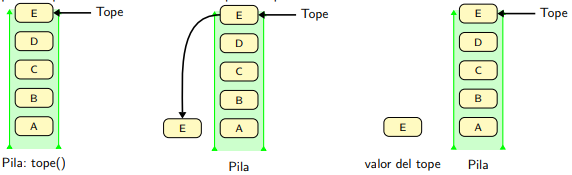
\includegraphics[width=0.8\textwidth]{diagrama1.png}
\caption{\label{fig:seq01}Ejemplo de un diagrama.}
\end{figure}


\begin{figure}[H]
\centering
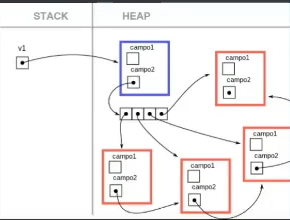
\includegraphics[width=0.8\textwidth]{diagrama2.png}
\caption{\label{fig:seq02}Otro ejemplo de un diagrama.}
\end{figure}


\end{document}
